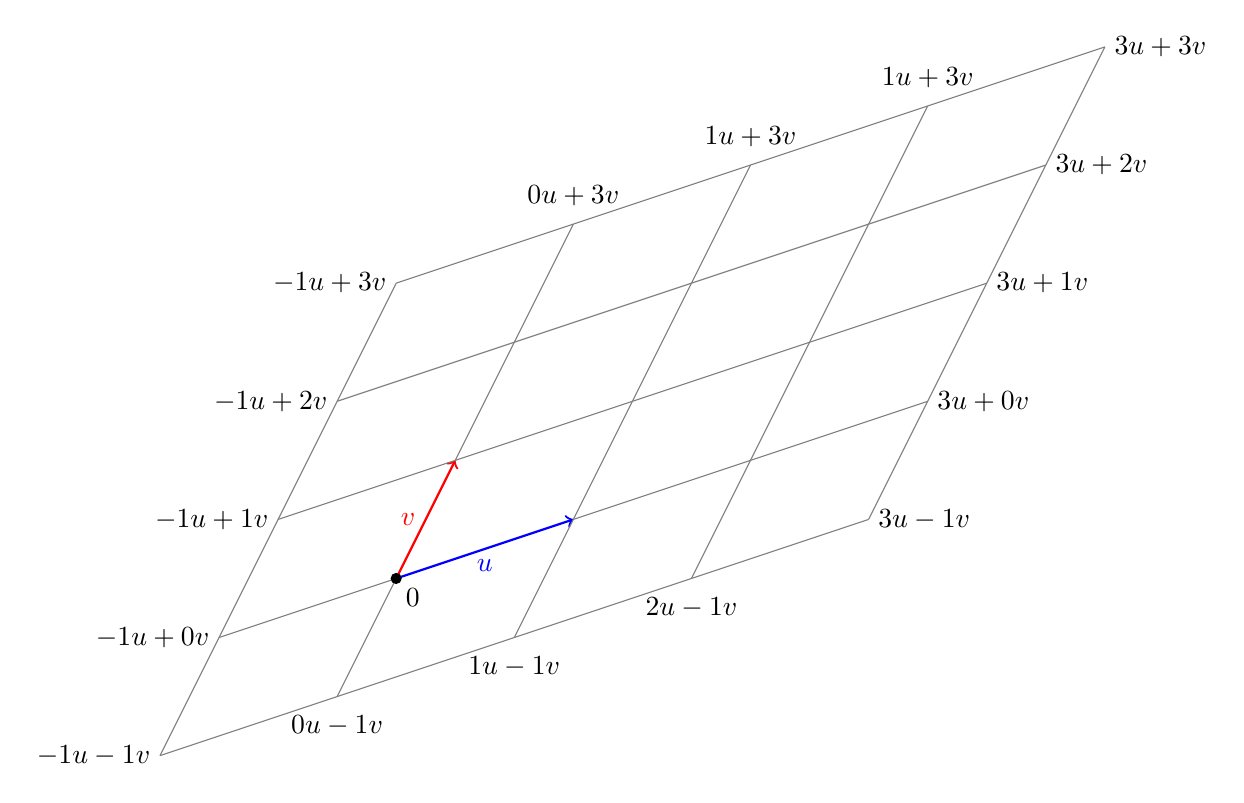
\begin{tikzpicture}[scale=1.5]
    \draw[->, thick, blue] (0,0) -- node[below]{$\vect{u}$} (1.5,0.5);
    \draw[->, thick, red] (0,0) -- node[left]{$\vect{v}$} (0.5,1);
    \draw[-, gray] (-2,-1.5)--(4,0.5);
    \draw[-, gray] (-1.5,-0.5)--(0,0);
    \draw[-, gray] (1.5,0.5)--(4.5,1.5);
    \draw[-, gray] (-1,0.5)--(5,2.5);
    \draw[-, gray] (-0.5,1.5)--(5.5,3.5);
    \draw[-, gray] (0,2.5)--(6,4.5);
    \draw[-, gray] (-2,-1.5)--(0,2.5);
    \draw[-, gray] (-0.5,-1)--(0,0);
    \draw[-, gray] (0.5,1)--(1.5,3);
    \draw[-, gray] (1,-0.5)--(3,3.5);
    \draw[-, gray] (2.5,0)--(4.5,4);
    \draw[-, gray] (4,0.5)--(6,4.5);
    \draw (-2.0,-1.5) node[left]{$-1\vect{u}-1\vect{v}$};
    \draw (-1.5,-0.5) node[left]{$-1\vect{u}+0\vect{v}$};
    \draw (-1.0,0.5) node[left]{$-1\vect{u}+1\vect{v}$};
    \draw (-0.5,1.5) node[left]{$-1\vect{u}+2\vect{v}$};
    \draw (0.0,2.5) node[left]{$-1\vect{u}+3\vect{v}$};
    \draw (1.5,3.0) node[above=0.75ex]{$0\vect{u}+3\vect{v}$};
    \draw (3.0,3.5) node[above=0.75ex]{$1\vect{u}+3\vect{v}$};
    \draw (4.5,4.0) node[above=0.75ex]{$1\vect{u}+3\vect{v}$};
    \draw (6.0,4.5) node[right]{$3\vect{u}+3\vect{v}$};
    \draw (5.5,3.5) node[right]{$3\vect{u}+2\vect{v}$};
    \draw (5.0,2.5) node[right]{$3\vect{u}+1\vect{v}$};
    \draw (4.5,1.5) node[right]{$3\vect{u}+0\vect{v}$};
    \draw (4.0,0.5) node[right]{$3\vect{u}-1\vect{v}$};
    \draw (2.5,0.0) node[below=0.75ex]{$2\vect{u}-1\vect{v}$};
    \draw (1.0,-0.5) node[below=0.75ex]{$1\vect{u}-1\vect{v}$};
    \draw (-0.5,-1.0) node[below=0.75ex]{$0\vect{u}-1\vect{v}$};
    \draw[fill] (0,0) circle [radius=1.2pt] node[below right]{$\vect{0}$};
  \end{tikzpicture}
